\part{Entrega 1}


\section{Introducción}
Las estructuras que se utilizan en el espacio deben contar con una serie de características que les permitan operar y cumplir con su función de forma eficiente y segura. Una de estas características es la relación de masa estructural y la longitud de la estructura con las frecuencias y modos de vibración de la misma. Si estos requisitos no se cumplen, mandar la estructura al espacio además de ser costoso, puede ser peligroso para la tripulación y la misión.

En este informe se estudiarán varias relaciones de masa estructural para obtener un área óptima de un reticulado, junto con la determinación de los modos de vibración que sean mayores a 0.1 Hz, ya que esta es una frecuencia que se considera segura en el espacio.

Para cumplir con este objetivo, se emplearán la librería OpenSeesPy para el análisis estructural y la identificación de las frecuencias y modos de vibración de la estructura, y PyVista para la visualización de los datos obtenidos.
\newpage
\section{Modelo}
Lo primero que se hizo para poder modelar de forma precisa, fue la creación de una función la cual permitiera la creación de un reticulado con las dimensiones y cantidad de vanos que el usuario deseara, que es el lo que se muestra a continuación:

\begin{lstlisting}
def conectar_nodos_cuadrado(node_tags, element_id, A, material_id, gamma, elements):
    for i in range(len(node_tags)):
        j = (i + 1) % len(node_tags)  # Cerrar el ciclo conectando el último con el primero
        #print(f'{i=}, {j=}')
        elements.append(crear_elemento_truss(element_id, node_tags[i], node_tags[j], A, material_id, gamma))
        element_id += 1

    #Ahora conecto una diagonal
    if node_tags[0] == 1:
        #Estoy en el primer elemento
        elements.append(crear_elemento_truss(element_id, node_tags[i], node_tags[j]+1, A, material_id, gamma))
        element_id += 1

    elif node_tags[-1] == num_capas*4 + 4:
        #Estoy en el ultimo elemento
        elements.append(crear_elemento_truss(element_id, node_tags[i], node_tags[j]+1, A, material_id, gamma))
        element_id += 1

    else:
        #Agrego dos diagonales
        elements.append(crear_elemento_truss(element_id, node_tags[i], node_tags[j]+1, A, material_id, gamma))
        element_id += 1

        elements.append(crear_elemento_truss(element_id, node_tags[i]-1, node_tags[j], A, material_id, gamma))
        element_id += 1
    return element_id
\end{lstlisting}

Así, los reticulados para 2, 4, 8 y 16 módulos se visualizan de la siguiente forma.

\begin{figure}[H]
    \begin{minipage}[b]{0.5\textwidth}
        \centering
        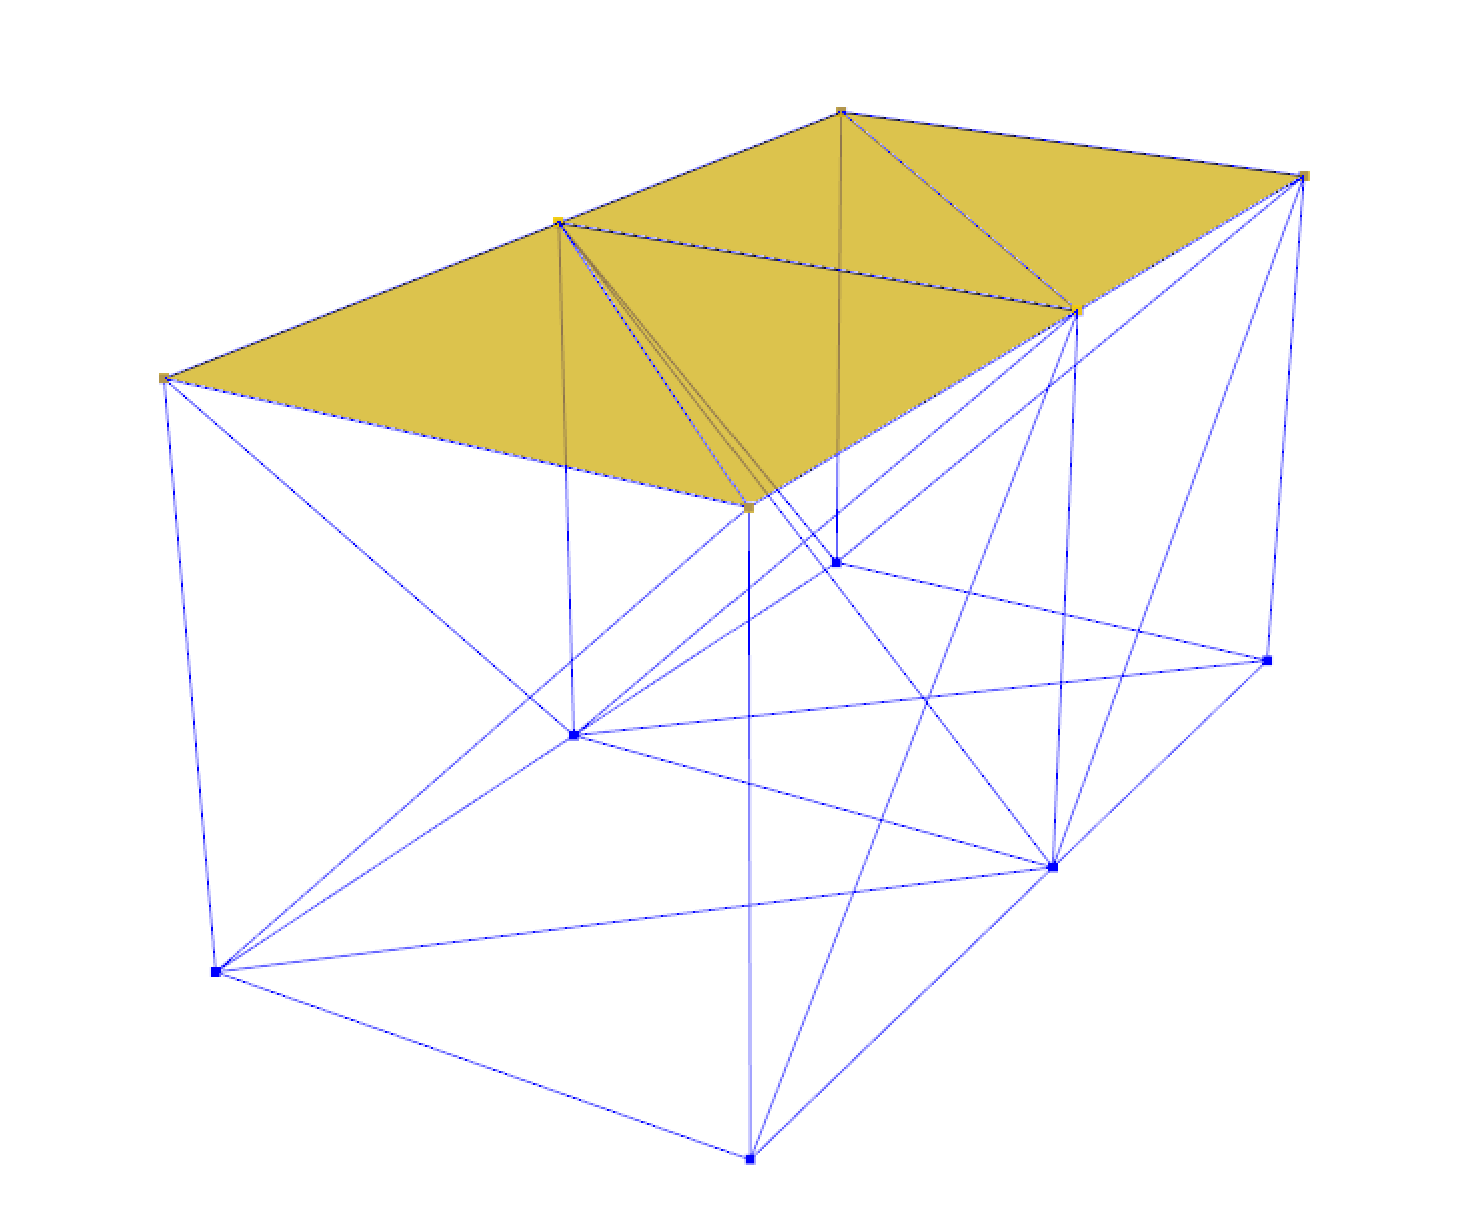
\includegraphics[width=\textwidth]{FOTOS/2.png}
        \caption{Reticulado de 2 módulos.}
    \end{minipage}
    \hfill
    \begin{minipage}[b]{0.5\textwidth}
        \centering
        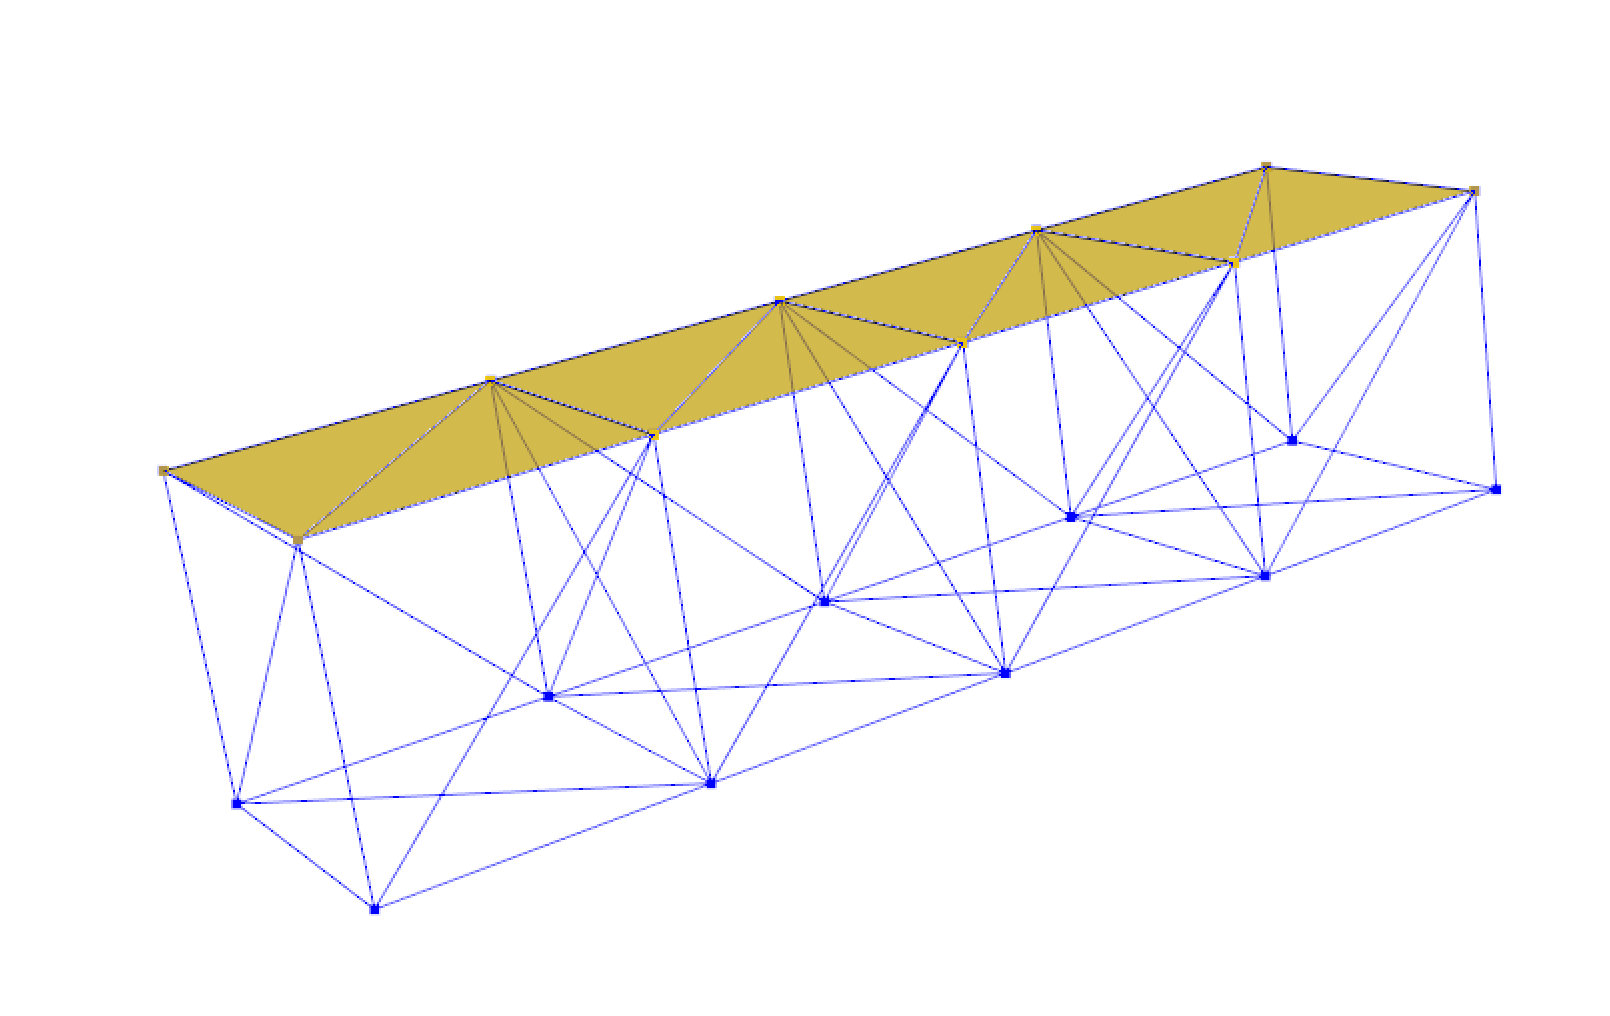
\includegraphics[width=\textwidth]{FOTOS/4.png}
        \caption{Reticulado de 4 módulos.}
    \end{minipage}
\end{figure}

\begin{figure}[H]
    \begin{minipage}[b]{0.5\textwidth}
        \centering
        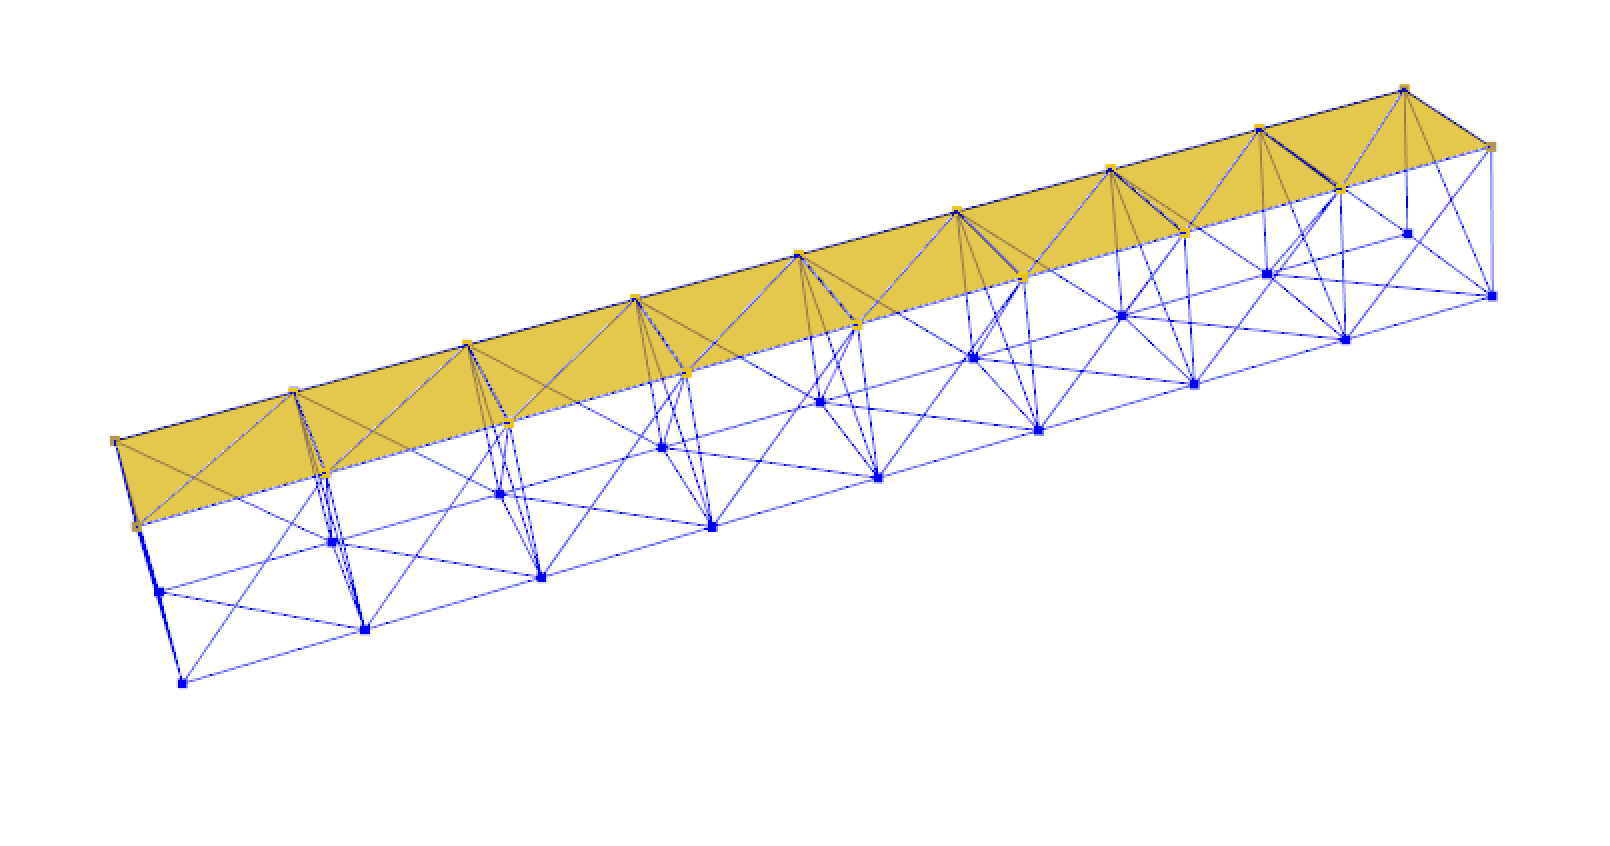
\includegraphics[width=\textwidth]{FOTOS/8.png}
        \caption{Reticulado de 8 módulos.}
    \end{minipage}
    \hfill
    \begin{minipage}[b]{0.5\textwidth}
        \centering
        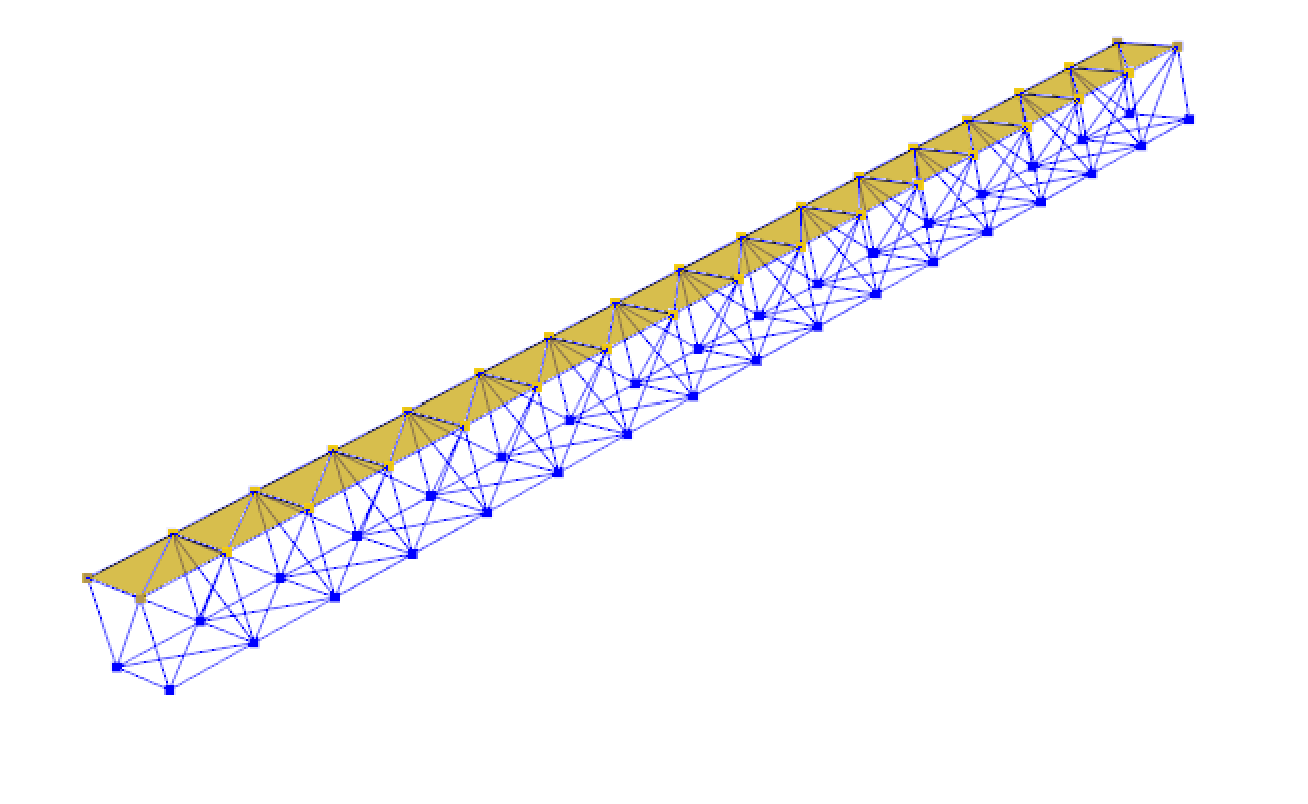
\includegraphics[width=\textwidth]{FOTOS/16.png}
        \caption{Reticulado de 16 módulos.}
    \end{minipage}
\end{figure}

Luego, se procedió a la obtención de las frecuencias y modos de vibración de la estructura, para lo cual se utilizó el comando \texttt{eigen} de OpenSeesPy. Con los datos obtenidos, se procedió a la visualización de los modos de vibración de la estructura, para lo cual se utilizó PyVista. A continuación, se muestran las estructuras con su deformación en el modo 1 de vibración, como ejemplo.

\begin{figure}[H]
    \begin{minipage}[b]{0.5\textwidth}
        \centering
        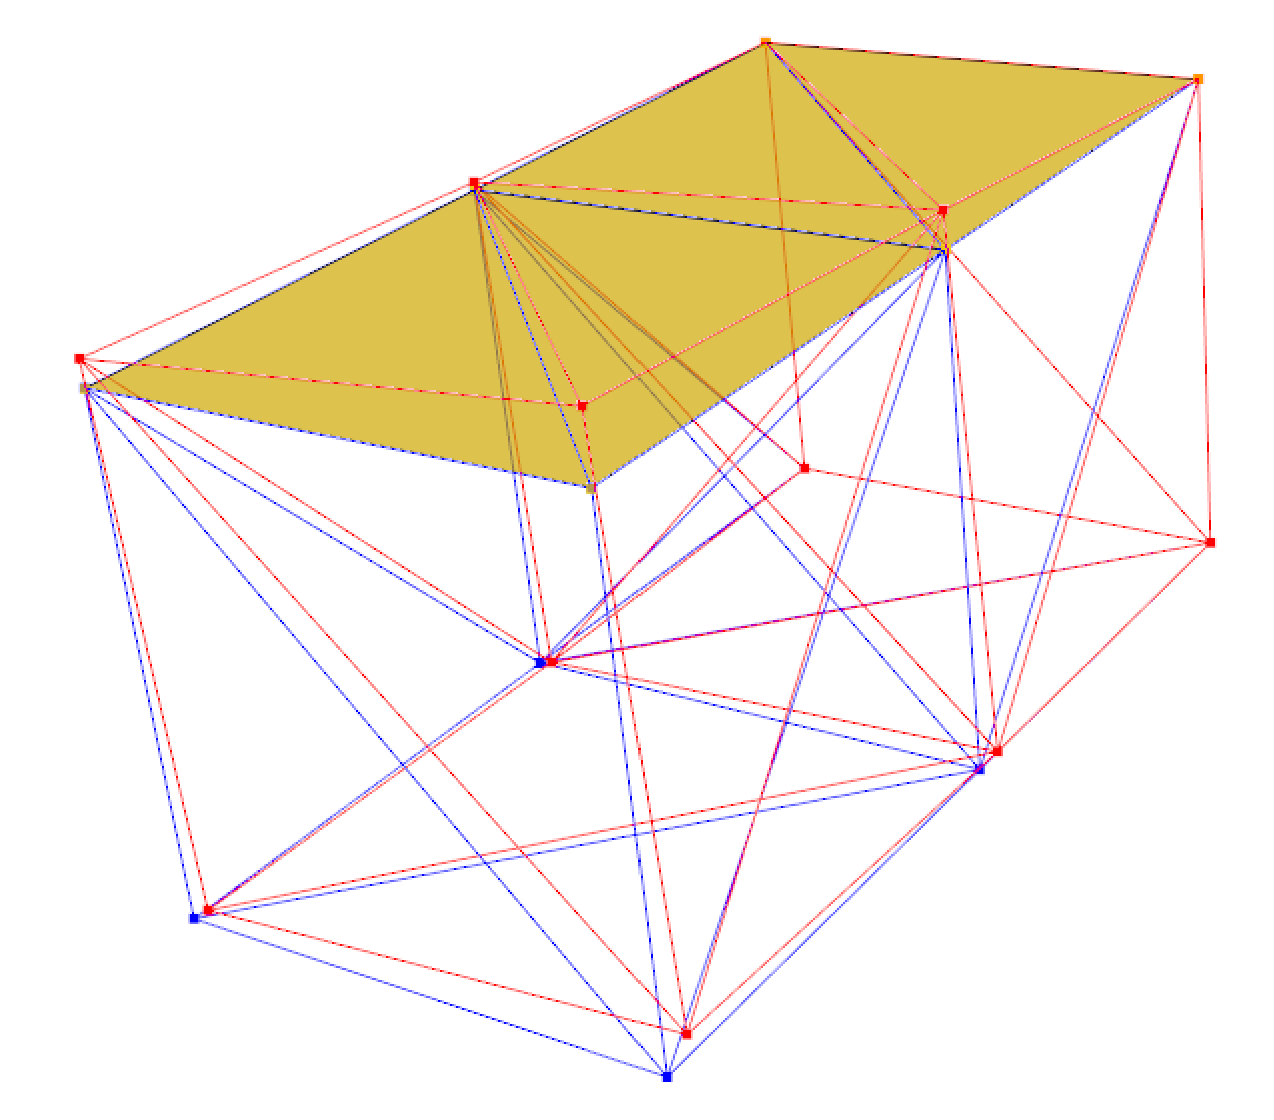
\includegraphics[width=\textwidth]{FOTOS/m1_2.png}
        \caption{Reticulado de 2 y su modo 1.}
    \end{minipage}
    \hfill
    \begin{minipage}[b]{0.5\textwidth}
        \centering
        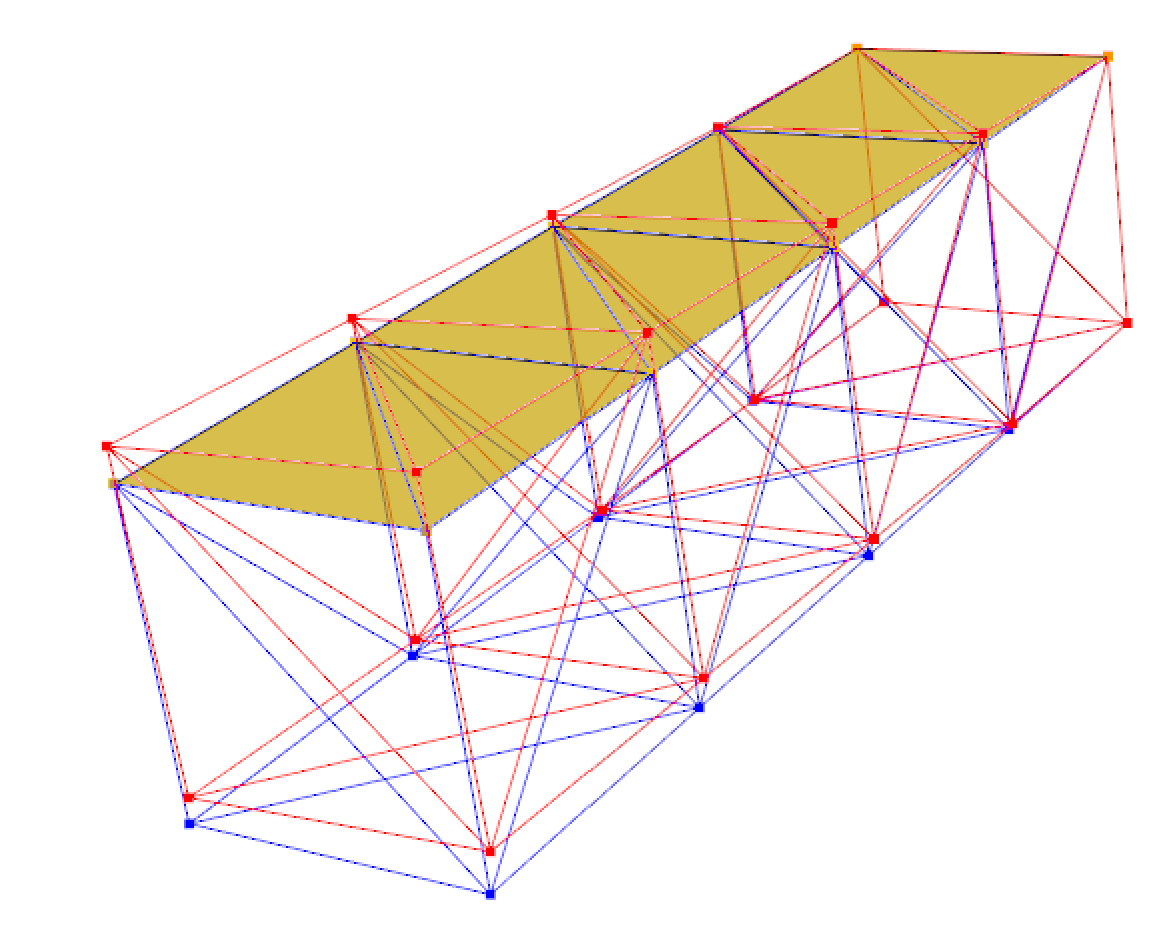
\includegraphics[width=\textwidth]{FOTOS/m1_4.png}
        \caption{Reticulado de 4 y su modo 1.}
    \end{minipage}
\end{figure}

\begin{figure}[H]
    \begin{minipage}[b]{0.5\textwidth}
        \centering
        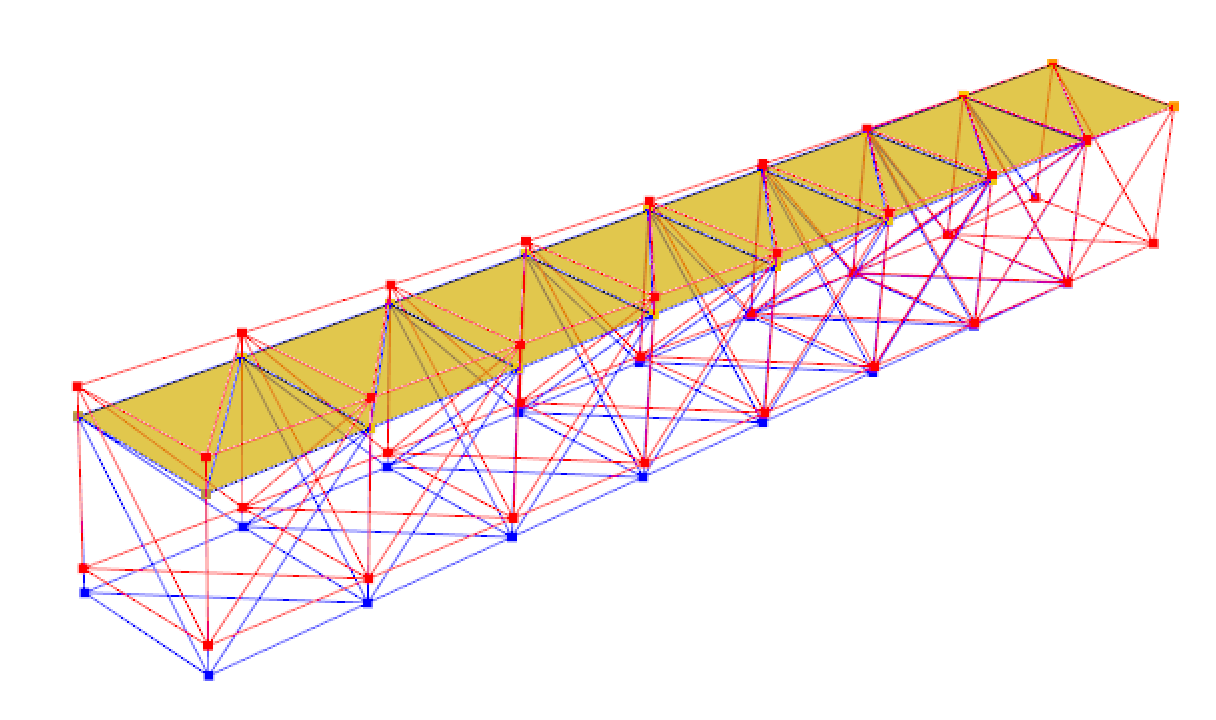
\includegraphics[width=\textwidth]{FOTOS/m1_8.png}
        \caption{Reticulado de 8 y su modo 1.}
    \end{minipage}
    \hfill
    \begin{minipage}[b]{0.5\textwidth}
        \centering
        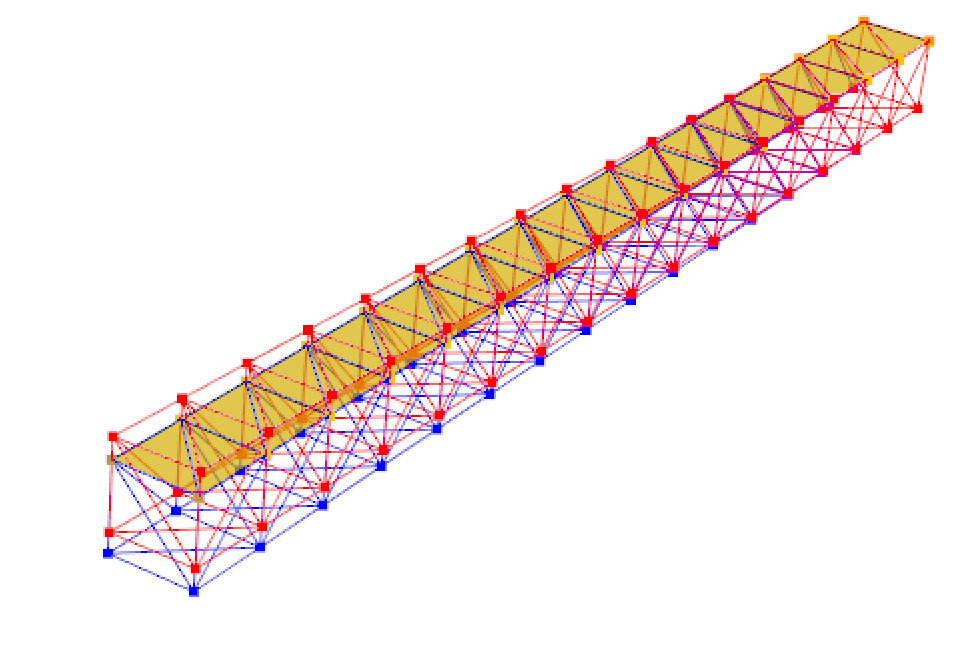
\includegraphics[width=\textwidth]{FOTOS/m1_16.png}
        \caption{Reticulado de 16 y su modo 1.}
    \end{minipage}
\end{figure}

Posteriormente, se procedió a calcular la relación de masa estructural con respecto a los paneles solares, para lo cual se utilizó la siguiente fórmula:

\begin{equation}
    \text{RME} = \frac{\text{Masa de la estructura}}{\text{Masa de los paneles solares}} \cdot 100
\end{equation}

Finalmente, se fueron calibrando los diámetros internos y externos de los tubos de la estructura, para obtener una relación de masa estructural que cumpliera con los siguientes porcentajes: 10\%, 20\%, 30\%


\section{Resultados}


\subsection{Caso de 2 vanos}
En el caso de 2 vanos se obtuvieron los siguientes diametros de las barras de fibra de carbono, además, se muestran los porcentajes de RME.

\begin{table}[H]
    \centering
    \begin{tabular}{cccc}
    \toprule
     A & Diametro exterior [mm] & Diametro interior [mm] & RME [\%] \\
    \midrule
     $A_{10\%}$ &  4 &  2.6 &  10.89 \\
     $A_{20\%}$ &  5 &  2.5 &  22.11 \\
     $A_{30\%}$ &  5.8 &  2.4 &  32.88 \\
    \bottomrule
    \end{tabular}
\end{table}

Donde se obtuvieron las siguientes frecuencias de vibración para cada porcentaje de RME.

\begin{table}[H]
    \centering
    \begin{tabular}{cccc}
    \toprule
     Frecuencia (Hz) & $A_{10\%}$ & $A_{20\%}$ & $A_{30\%}$ \\
    \midrule
     0 &  0.245 &  0.349 &  0.425 \\
     1 &  0.283 &  0.400 &  0.484 \\
     2 &  0.314 &  0.445 &  0.540 \\
     3 &  0.666 &  0.947 &  1.154 \\
     4 &  0.673 &  0.958 &  1.166 \\
     5 &  0.744 &  1.054 &  1.280 \\
     6 &  1.014 &  1.442 &  1.757 \\
     7 &  1.046 &  1.488 &  1.812 \\
     8 &  1.206 &  1.717 &  2.092 \\
     9 &  1.454 &  2.070 &  2.522 \\
    \bottomrule
    \end{tabular}
\end{table}

\subsection{Caso de 4 vanos}
En el caso de 4 vanos se obtuvieron los siguientes diametros de las barras de fibra de carbono, además, se muestran los porcentajes de RME.

\begin{table}[H]
    \centering
    \begin{tabular}{cccc}
    \toprule
     A & Diametro exterior [mm] & Diametro interior [mm] & RME [\%] \\
    \midrule
     $A_{10\%}$ &  4 &  2.6 &  10.41 \\
     $A_{20\%}$ &  5 &  2.5 &  21.13 \\
     $A_{30\%}$ &  5.8 &  2.4 &  31.41 \\
    \bottomrule
    \end{tabular}
\end{table}

Donde se obtuvieron las siguientes frecuencias de vibración para cada porcentaje de RME.

\begin{table}[H]
    \centering
    \begin{tabular}{cccc}
    \toprule
     Frecuencia (Hz) & $A_{10\%}$ & $A_{20\%}$ & $A_{30\%}$ \\
    \midrule
     0 &       0.103 &       0.146 &       0.175 \\
     1 &       0.141 &       0.195 &       0.228 \\
     2 &       0.162 &       0.228 &       0.272 \\
     3 &       0.342 &       0.486 &       0.582 \\
     4 &       0.393 &       0.553 &       0.656 \\
     5 &       0.449 &       0.633 &       0.754 \\
     6 &       0.597 &       0.849 &       1.015 \\
     7 &       0.624 &       0.887 &       1.060 \\
     8 &       0.688 &       0.974 &       1.162 \\
     9 &       0.735 &       1.039 &       1.236 \\
    \bottomrule
    \end{tabular}
\end{table}


\subsection{Caso de 8 vanos}
En el caso de 8 vanos se obtuvieron los siguientes diametros de las barras de fibra de carbono, además, se muestran los porcentajes de RME.

\begin{table}[H]
    \centering
    \begin{tabular}{cccc}
    \toprule
     A & Diametro exterior [mm] & Diametro interior [mm] & RME [\%] \\
    \midrule
     $A_{10\%}$ &  4 &  2.6 &  10.17 \\
     $A_{20\%}$ &  5 &  2.5 &  20.63 \\
     $A_{30\%}$ &  5.8 &  2.4 &  30.68 \\
    \bottomrule
    \end{tabular}
\end{table}

Donde se obtuvieron las siguientes frecuencias de vibración para cada porcentaje de RME.

\begin{table}[H]
    \centering
    \begin{tabular}{cccc}
    \toprule
     Frecuencia (Hz) & $A_{10\%}$ & $A_{20\%}$ & $A_{30\%}$ \\
    \midrule
     0 &       0.035 &       0.049 &       0.059 \\
     1 &       0.064 &       0.083 &       0.095 \\
     2 &       0.081 &       0.115 &       0.139 \\
     3 &       0.147 &       0.208 &       0.253 \\
     4 &       0.195 &       0.266 &       0.314 \\
     5 &       0.234 &       0.330 &       0.399 \\
     6 &       0.307 &       0.435 &       0.528 \\
     7 &       0.336 &       0.474 &       0.574 \\
     8 &       0.388 &       0.548 &       0.663 \\
     9 &       0.444 &       0.629 &       0.760 \\
    \bottomrule
    \end{tabular}
\end{table}


\subsection{Caso de 16 vanos}
En el caso de 16 vanos se obtuvieron los siguientes diametros de las barras de fibra de carbono, además, se muestran los porcentajes de RME.

\begin{table}[H]
    \centering
    \begin{tabular}{cccc}
    \toprule
     A & Diametro exterior [mm] & Diametro interior [mm] & RME [\%] \\
    \midrule
     $A_{10\%}$ &  4 &  2.6 &  10.05 \\
     $A_{20\%}$ &  5 &  2.5 &  20.39 \\
     $A_{30\%}$ &  5.8 &  2.4 &  30.32 \\
    \bottomrule
    \end{tabular}
\end{table}

Donde se obtuvieron las siguientes frecuencias de vibración para cada porcentaje de RME.

\begin{table}[H]
    \centering
    \begin{tabular}{cccc}
    \toprule
     Frecuencia (Hz) & $A_{10\%}$ & $A_{20\%}$ & $A_{30\%}$ \\
    \midrule
     0 &       0.010 &       0.014 &       0.017 \\
     1 &       0.025 &       0.029 &       0.031 \\
     2 &       0.040 &       0.057 &       0.069 \\
     3 &       0.052 &       0.074 &       0.090 \\
     4 &       0.086 &       0.112 &       0.130 \\
     5 &       0.113 &       0.160 &       0.194 \\
     6 &       0.130 &       0.184 &       0.223 \\
     7 &       0.161 &       0.222 &       0.264 \\
     8 &       0.192 &       0.270 &       0.326 \\
     9 &       0.212 &       0.299 &       0.363 \\
    \bottomrule
    \end{tabular}
\end{table}



\section{Conclusiones}